 Urbanisation and globalisation are terms that have been used more and more frequently. Various studies show that countries around the world are experiencing rapid growth in population figures, especially in urban areas. In 2009, it was concluded that more than 50\% of the world's population resides in urban areas. By 2015, this figure increased to 53\% and researchers predict this figure to increase to 68\% by 2050 \citep{moreno2016urbanization}. Rapid urbanization is defined as one of the mega-trends, along with e-commerce, that will reshape city logistics as we know it. The increase in population concentration in urban areas, coupled with a demanded increase in customer service levels, has resulted in more complex city logistics scenarios. This emphasises the need for well-managed city logistics to ensure the demands of all urban residents are satisfied, while simultaneously developing the economy.\par

%------------------------------------------------------------------------------------------------------------------------------------------------------------------------------------------------------------------------------------
\section{City logistics in urban areas}
 Transportation planning has become a factor to consider when attempting to control the number of vehicles in urban areas. In the past, city planning in urban areas focused mainly on planning and controlling passenger transport. However, achieving sustainable urban freight transport requires the inclusion of all actors utilising the road and traditional strategic planning procedures no longer deem sufficient. As a result, the focus has been shifted towards strategically planning freight vehicles as these vehicles play an important role in transportation systems \citep{bean2018}.

During the last decade, logistic practitioners have introduced new transportation methods and services, such as e-commerce, last-mile deliveries as well as speedy deliveries, in an attempt to improve the customers' experience. However, the aftermath of its inclusion accelerated the negative impacts of the existing complex obstacle - urbanization. Population growth and improved customer service both lead to an increase in the number of vehicles on the road. Important environmental impacts include the negative impacts of emissions, noise pollution and a variety of social impacts including an increase in congestion, road accidents and public health concerns \citep{gonzalez2012defining}. These phenomena resulted in a growing interest in research topics that consider sustainable transportation and innovative logistic solutions to address these concerns. \par
 
The expansion of cities is currently viewed as one of the most crucial research topics to investigate \citep{figiel2014development} as current urban logistic practices in megacities exhibit the absence of state-of-the-art transportation planning initiatives. Research identifies cross-company cooperation as a mature means of moving towards more sustainable logistic practices.  

%According to \citet{jennings2017planning}, the consequences of urban freight movements in sub-Saharan African countries have not received the required attention. A review of the current urban logistics practices, specifically focusing on literature concerning the development of urban freight transport concepts, investigated the sustainability of these solutions in 21 megacities across the globe. Each of the reviewed articles failed to achieve a satisfactory sustainability figure, when ranked against the cities' Ecology-, Economy- and Social ranking. These indicators evaluated the cities' Ecological impact (green gas emissions, etc.), the Economical impact (the number of cars, ride time to work, etc) and the Social impact (traffic accidents, noise exposure, population density, etc).  The study concluded by emphasizing the need for integrated solutions that require the participation of all the affected stakeholders. The most viable solution to improve the logistic processes in mature-, transitional- and emerging cities, was given as cross-company cooperation \citep{figiel2014development}. \par

Cooperative initiatives motivate stakeholders to consider the impacts of certain decisions made from a holistic view. The focus is turned towards all the affected participants in the supply chain, rather than focusing on its individual advances. \par



% Add an image of the different actors in the supply chain and how they interact

When referring to the freight transportation industry, cooperation between the different stakeholders entail the improvement and optimisation of the logistic activities in urban areas by synchronising deliveries and resource sharing.\par

%----------------------------------------------------------------------------------------------------------------------------------------------------------------------------------------------------------------------------------------------------
\section{Collaboration in urban freight transportation}
%The benefits of cross-company cooperation lie in the potential to increase the load factors of freight vehicles while simultaneously reducing the number of empty trips \citep{figiel2014development}. This is done by grouping smaller loads destined for a certain location. 

Collaboration in transport is a well-known topic with a large body of literature on urban freight collaboration. \citet{lindawati2014collaboration} identified the factors influencing potential collaborators to participate in coalitions. The main motivation was recognised as the expected benefits gained from participating as it encourages different stakeholders to change their behaviour. As for the barriers, the risks of losing their competitive intelligence was regarded as the most substantial factor influencing the participation decision. Other, less effective barriers, include the internal capability of the different stakeholders to meet the requirements of the urban logistics and the trust between participants.\par

The importance of estimating and allocating these benefits is evident in literature. Various articles by researchers such as \citet{lozano2013cooperative,houghtalen2007designing,defryn2013gain,dai2012profit,audy2012empirical} have focused their energy towards the investigation of improved methods to estimate collaboration benefits and state-of-the-art models to allocate these benefits.
The advantages of collaborating is not limited to the reduction in the delivery costs but extends to reducing the number of vehicles on the road, increasing the accompanied vehicle load factors  \citep{janjevic2018investigating} and reducing the overall supply chain cost \citep{lozano2013cooperative}.\par
 
 Even though the benefits from collaborating are well known, the implementation of collaboration initiatives has a high failure rate. In a study done by \citet{quak2008sustainability}, more than half of the implemented initiatives failed at the proposal or implementation phase. The main factors contributing to the high failure rate and resistance to collaborate was the fear of losing competitiveness and the uncertainty of the expected benefits \citep{lindawati2014collaboration}. These findings are echoed by \citet{ozener2008allocating} in his study on cost allocations in a coalition. The uncertainty of the expected benefits and the risk of failure is higher if the collaboration models used to quantify and allocate the benefits are complex and difficult to understand. Collaboration's success relies on the participation of all parties involved. As the participation of the different stakeholders is fueled by the gained benefits, it has a direct impact on the success of the collaboration. Therefore, the methods used to estimate and allocate these benefits is of utmost importance. \par


Literature provides various methods to allocate the benefits in a collaboration, however, allocating the cost between participants is not an easy task \citep{lozano2013cooperative}. The stability of the coalition relies heavily on the guarantee that the benefits will be divided fairly and equally between the participants. Past research on cost allocation methods provides different mathematical models to equally share the benefits amongst participants \citep{lozano2013cooperative}. The literature identifies more than 40 existing methods, with a large portion, including concepts of Cooperative Game Theory. The existing literature on cost allocation methods exhibits the success of incorporating game theory concepts in the development of new methods. Understanding the application of these methods is, however, not evident in current research. The cost allocation methods proposed by skilled researchers in the field, are not based on the requirements of actual transportation systems in practical scenario's but are rather theoretical based methods of high complexity \citep{ozener2008allocating}. Deploying many of these models in industry would deem difficult due to its complexity. Therefore, a model that theoretically performs well based on experiments, would not necessarily survive when implemented in the transportation industry.
%A framework based on practical scenarios will allow the user to address real-world problems as it represents different individuals that make the decision to participate in the collaboration \citep{lozano2013cooperative}. 


%----------------------------------------------------------------------------------------------------------------------------------------------------------------------


%------------------------------------------------------------------------------------------------------------------------------------------------------------------------------------------------------------------------------------
\section{Potential contributions to existing literature }

Even though the existing literature is available, potential participants and decision-makers in the urban transportation sector remain hesitant to attempt a collaboration with other stakeholders. This is due to the uncertainty of the outcomes and how benefits will be equally shared. However, another influence contributing to the reluctance is the complexity of the cost allocation methods found in the literature. Although these methods are verified and approved by researchers, the practical implementation thereof seems impossible for practitioners attempting collaborative initiatives. This forces stakeholders to fall back to old, less efficient cost allocation methods. This can be addressed by introducing a practical tool that has the potential to integrate the complex cost allocation models into a simulation that is easy to implement in real-life scenarios. The need for a tool that can provide a close-to-reality simulation to estimate, measure and distribute the benefits gained from the collaboration, was also identified by \citet{cruijssen2007horizontal}.\par

This paper identified three objectives that were found as being lacking or incomplete in literature:
\begin{enumerate}
    \item Receiver driven collaborations have only recently been addressed in the literature. As the receiver has the power to directly influence the delivery schedule, it is worthwhile to investigate a receiver driven collaboration and identify areas where the use of such a collaboration model can be expanded.
    
    
    \item The cost allocation method used to distribute the savings amongst the members of the coalition, plays a vital role in the forming and continuity of the collaboration. Literature on cost allocation models is complex and difficult to understand. This contributes to the hesitance to form a collaboration in the freight transportation industry. The second contribution aims to identify a cost allocation method available in the literature that appeals to individuals in the transportation industry, whilst yielding sufficient results.
    
    %This emphasizes the need for a practical tool that would present collaboration as an appealing method to stakeholders in different supply chains. Convincing potential partners to join a coalition could be simplified if the estimated benefits and the methods used to allocate these benefits, was displayed on a platform that visually presented the results in a validated, trustworthy and understandable manner. A simulation tool could assist in achieving this as it offers a means of simulating close-to-reality scenarios.
    
    \item A simulation tool could assist in convincing potential stakeholders to form part of the collaboration as it offers a means of simulating a close-to-reality scenario. Convincing potential partners to join a coalition could be simplified if the estimated benefits and the methods used to allocate these benefits, was displayed on a platform that visually presented the results in a validated, trustworthy and understandable manner.
    
    %A simulation tool assists in convincing potential stakeholders to form part of the collaboration as it offers a means of simulating a close-to-reality scenario. Such a tool could assist in estimating and fairly distributing these benefits, according to the selected cost allocation mathematical model. The third contribution will, therefore, evaluate the practical implementation of the tool when applied by stakeholders in the freight transport industry. The ease of implementation and functionality as a decision support tool will be assessed.
\end{enumerate}

Urbanization is inevitable. In recent years, the importance of planning freight vehicles has captured the attention of many researchers. Collaboration serves as a sustainable method to reduce the number of vehicles on the road. However, forming and implementing collaborations in urban freight transportation still poses barriers when attempted in industry.
%The limitations found in the literature will be addressed by focusing on a receiver-driven collaboration. The paper will aim to propose a practical solution by integrating an existing cost allocation tool, that could potentially be used in real-life scenarios, into a simulation tool.  This could enable potential collaborators to test different scenarios before entering the collaboration and increase the attractiveness of cross-company collaborations.\par

%---------------------------------------------------------------------------------------------------------------------------------------------------------------------------------------
\section{Problem Statement}
Rapid urbanization has emphasised the need for sustainable urban logistics practices, where collaborative freight transportation serves as a sufficient candidate. Collaboration in urban freight planning yields numerous benefits, however, the potential participants' resistance to collaborate still poses a barrier to implement successful collaborations. This is mainly due to the uncertainty of the expected benefits which is further fueled by the complexity of the mathematical models from which they are derived. Therefore, there is a need for a practical tool that could estimate the expected benefits gained from a collaboration whilst simplifying the computational complexity of cost allocation methods. This need is echoed by, \citet{cruijssen2007horizontal} that suggests the use of a simulation tool to evaluate the expected results and impacts of different collaborations before entering the coalition. Such models have been proposed by BEAN and \citet{schroeder2012towards}. It is however noted that these models are limited. A thorough investigation is required to identify the models currently available in literature, to identify the shortcomings and further refine these models. \par

%Agent-based modelling (\acrshort{abm}) is a simulation technique that has the capability of incorporating interactions and individual actions between different agents \citep{anand2014ontology}. As the receiver generates the demand for the delivery of goods, the inclusion of the receiver agent in the collaboration could assist in conceptualising the emergent behaviours of the affected agents in the collaboration.\par

Based on the problem at hand, the following research question was identified:

\textit{How can the current infrastructure of modelling urban freight collaborations be refined to assist decision-makers, in urban areas, in estimating and allocating benefits gained from a receiver-driven collaboration in a way that is easy to understand and apply in real-life scenarios?}



%----------------------------------------------------------------------------------------------------------------------------------------------------------------------------------------------------------------------------------------
\section{Research design}

The aim of this dissertation is to support the inclusion of collaboration between urban freight vehicles in daily deliveries.  Although the concept of collaboration is not new, there are still a number of barriers that prevent its inclusion. The estimation and allocation of costs during collaboration serves as one of the largest barriers to overcome as it is the key element that motivates players to form part of the coalition.  The literature identifies a large number of existing cost allocation methods, where the majority of these models are based on Cooperative Game Theory concepts. A cost allocation method will be selected amongst the existing models. The selection process will not solely focus on the performance of the cost allocation method in literature, but will also consider the ease of implementing and applying the model in the urban freight transport industry. The aim is to provide a solution that balances the theoretical knowledge obtained by research experts with the requirements and capabilities of practitioners in the field. By minimising the gap between theory and reality, one can obtain a model that appeals to the members of the transport industry, but also incorporates the fundamentals of mathematical modelling and state-of-the-art principles and software.

%The aim of this dissertation is twofold.
%The theoretical aspect of the problem, which is the integration of a cost allocation method into a simulation tool, is addressed. The literature identifies a large number of existing cost allocation methods where the majority of these models are based on Cooperative Game Theory concepts. A cost allocation method will be selected amongst the existing models. The cost allocation method will be included in a simulation tool where it is available to decision-makers exploring collaborative scenarios.

%The second contribution assesses the practical implementation of the developed model. The simulation model will focus on the interaction between the receiver and the carrier agent. A case study will assess the practical implementation of the model developed, to determine if the model can be used by carrier agents, as a decision support tool. The tool will assist in optimising fleet composition, calculating the benefits from the collaboration and determining the allocation of benefits amongst the actors involved.

\section{Research Methodology}
The research methodology used in this dissertation was proposed by \citet{vaishnavi2004design}. It is considered a generally accepted method among researchers and appeared in numerous studies including \citet{bean2020behavioural,alfrijat2009a}. It consists of five process steps as depicted in figure \ref{fig:method_steps}.

\begin{figure}[ht]
    \centering
    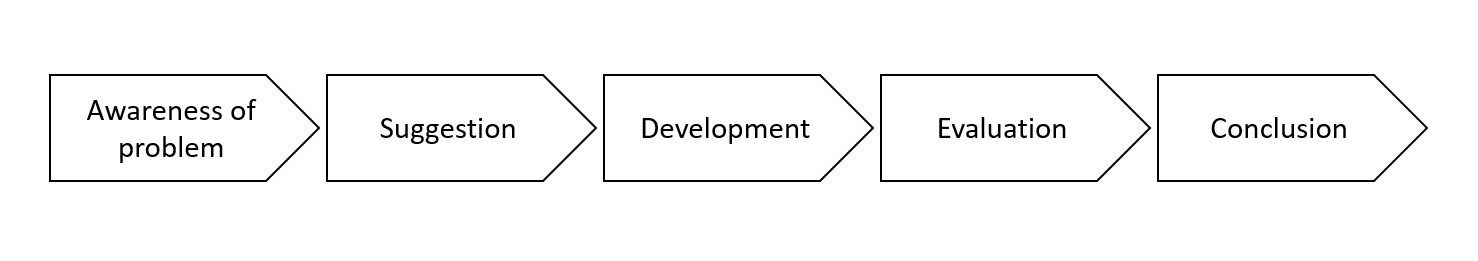
\includegraphics[width=1\textwidth]{images/Method_steps.PNG}
    \caption{Research Methodology Process Steps}
    \label{fig:method_steps}
\end{figure}

\paragraph{Awareness of Problem:} This is the identification of a problem, or multiple problems, within a certain discipline. The output from this process step identifies an opportunity to contribute new findings to the specific research field \citep{vaishnavi2004design}. During this step, the relevant information is gathered to understand the problem at hand. From here, additional information is gathered to conceptualise a means of solving the identified problem \citep{alfrijat2009a}.
The review will include an investigation into the existing methods applied to modelling urban freight transportation. From here, the models that include the logistic behaviour of the different stakeholders will be investigated, as this is an important consideration when modelling collaborations. This will be done by conducting a literature review in Chapter \ref{chapter2}. Alternative cost allocation methods found in the literature are investigated, to identify a single method of choice. This selection will be based on the success rate of the method and the ease of implementation. The literature review concludes with a detailed discussion on the current state ,and shortcomings, of research in the field of logistic behavioural modelling.  \par

\paragraph{Suggestion:} Once an awareness of the problem is achieved, the suggestion step is addressed. Suggestion is a form of tentative design \citep{alfrijat2009a,vaishnavi2004design}. This process step is completed in Chapter \ref{chapter 3}. This chapter will provide a deeper understanding of the model framework to ensure the suggested approach fits within the development requirements of this platform. The main output from this step is the formulation of an additional cost allocation method and the proposed methodology to embed the model into a simulation platform, such as \acrshort{matsim}. The available modules within the platform will be utilised to evaluate the performance of the additional cost allocation model. 

\paragraph{Development:} During this process step the tentative design is further developed and implemented. The shortcomings identified in Chapter \ref{chapter2} and the suggested solution approach discussed in Chapter \ref{chapter 3} are developed.
During this step, the cost allocation model will be developed. The main output from this step is the inclusion of an additional cost allocation method, selected in Chapter \ref{chapter2}, that evolves the current state of modelling collaborations to a more realistic representation of the freight transportation in urban areas.\par

\paragraph{Evaluation:} During the evaluation step, the artefact is evaluated according to specified criteria to determine if it performs as expected. Deviations from the expected behaviour are analysed to determine the source of the deviation. The evaluation phase is discussed in Chapter \ref{chapter 5}. The accuracy of the cost allocation method is examined to evaluate the performance of the model against expected results, to ensure the model behaves as predicted. Once satisfactory results are achieved, the usability and applicability of the model is evaluated to identify the shortcomings that prohibit the model from simulating close-to-reality collaboration scenarios.

\paragraph{Conclusion:} The conclusion phase reports on the performance of the artefact. It consolidates the knowledge gained and reports on the success of answering the research question provided. Shortcoming identified in the performance of the model serve as areas for future research in the discipline area. The consolidated research results, knowledge gained and opportunities for further research is concluded in Chapter \ref{chapter 6}.


%------------------------------------------------------------------------------------------------------------------------------------------------------------------------------------------------------------------
\section{Expected contribution}
 Rapid urbanisation emphasises the need for well-managed city logistics. Decision-makers need to turn towards sustainable urban freight transportation systems, such as collaboration in freight vehicles, to improve their current logistic practises. 
 In this dissertation the current state of research on logistic behavioural modelling, or more specifically the modelling of receiver-driven collaborations, is investigated to identify the shortcomings of applying the knowledge gained by research in practical scenarios. Forming a coalition has many challenges and barriers that hinder the application of collaboration amongst urban freight vehicles. One of the main barriers identified in research is the estimation and allocation of the costs amongst the coalition members. Although the literature presents a substantial amount of research on cost allocation methods, the application of these methods are not as evident in practise. Decision-makers in the transportation industry still consider the estimation and allocation of benefits gained, as a barrier to overcome. Cost allocation models are based on concepts of Cooperative Game Theory that are complex and difficult to understand. The contribution of this dissertation is thus the inclusion of a cost allocation method in a simulation tool that allows the modelling of. 
 
 %-----------------------------------------------------------------------------------------------------------------------------------------------------------------------------------------------------------------------